\section{Proposed Method}
\label{sec:proposed_method}

The framework combines a random-subspace Random Forest (RF) point predictor, RP-aware validation, final training on all RPs, and conformal uncertainty regions computed from RP-grouped residuals (Fig.~\ref{fig:overall_framework}).

\begin{figure*}[!t]
	\centering
	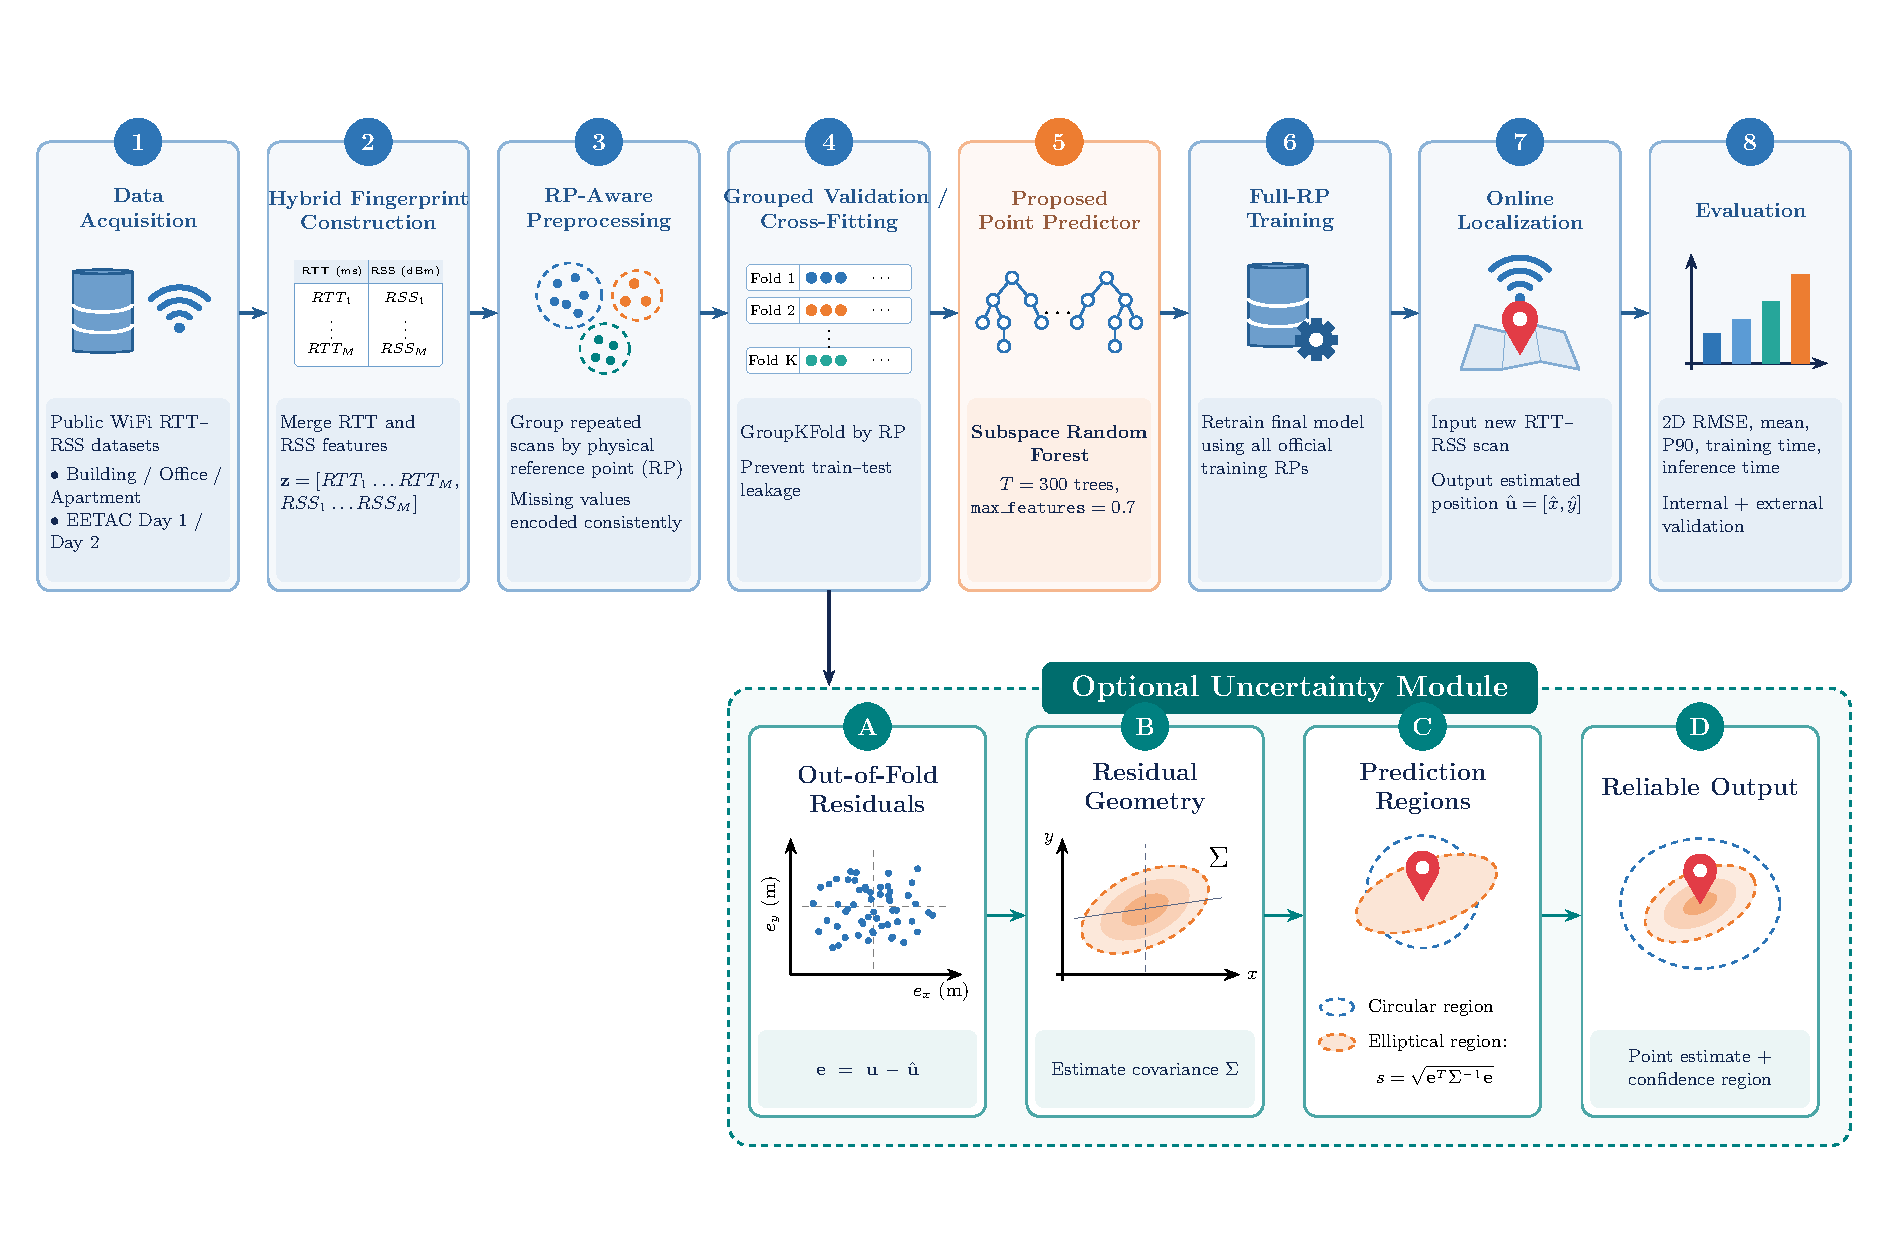
\includegraphics[width=\textwidth]{figures/methodology/fig02_framework.pdf}
	\caption{Overall workflow of the proposed hybrid Wi-Fi RTT--RSS indoor localization framework. Hybrid RTT and RSS measurements are first organized into fingerprint vectors and grouped according to their physical reference-point coordinates. A random-subspace Random Forest is used for point localization, while grouped out-of-fold residuals characterize positioning uncertainty. The final localization model is trained using all available training reference points.}
	\label{fig:overall_framework}
\end{figure*}

% ============================================================
\subsection{Random-Subspace Hybrid RTT--RSS Random Forest}
\label{subsec:subspace_rf}

An RF regressor consists of $T$ trees $h_t:\mathbb{R}^{p}\rightarrow\mathbb{R}^{2}$, each grown on a bootstrap sample of $\mathcal{D}$, and predicts
\begin{equation}
	\hat{\mathbf{u}}
	=
	f(\mathbf{z})
	=
	\frac{1}{T}\sum_{t=1}^{T}h_t(\mathbf{z}).
	\label{eq:rf_prediction}
\end{equation}
At every node, the split is chosen among a random subset of $m_{\mathrm{try}}$ of the $p$ features,
\begin{equation}
	m_{\mathrm{try}}
	=
	\max\left(1,\lfloor \rho p\rfloor\right),
	\qquad \rho\in(0,1].
	\label{eq:mtry}
\end{equation}
The full-feature configuration used in prior hybrid RTT--RSS work, $\rho=1$, is bagging of regression trees: the only source of diversity is the bootstrap sample, and the same dominant features can shape most splits of most trees. Hybrid fingerprints make this costly, because the RTT and RSS of one AP and the measurements of neighboring APs carry overlapping spatial information, while NLOS propagation and visibility changes make individual features intermittently unreliable. The proposed configuration uses $\rho=0.7$ and $T=300$ (Fig.~\ref{fig:rf_subspace}). The deployed model remains a single $T$-tree ensemble evaluated by Eq.~\eqref{eq:rf_prediction}.

\begin{figure*}[!t]
	\centering
	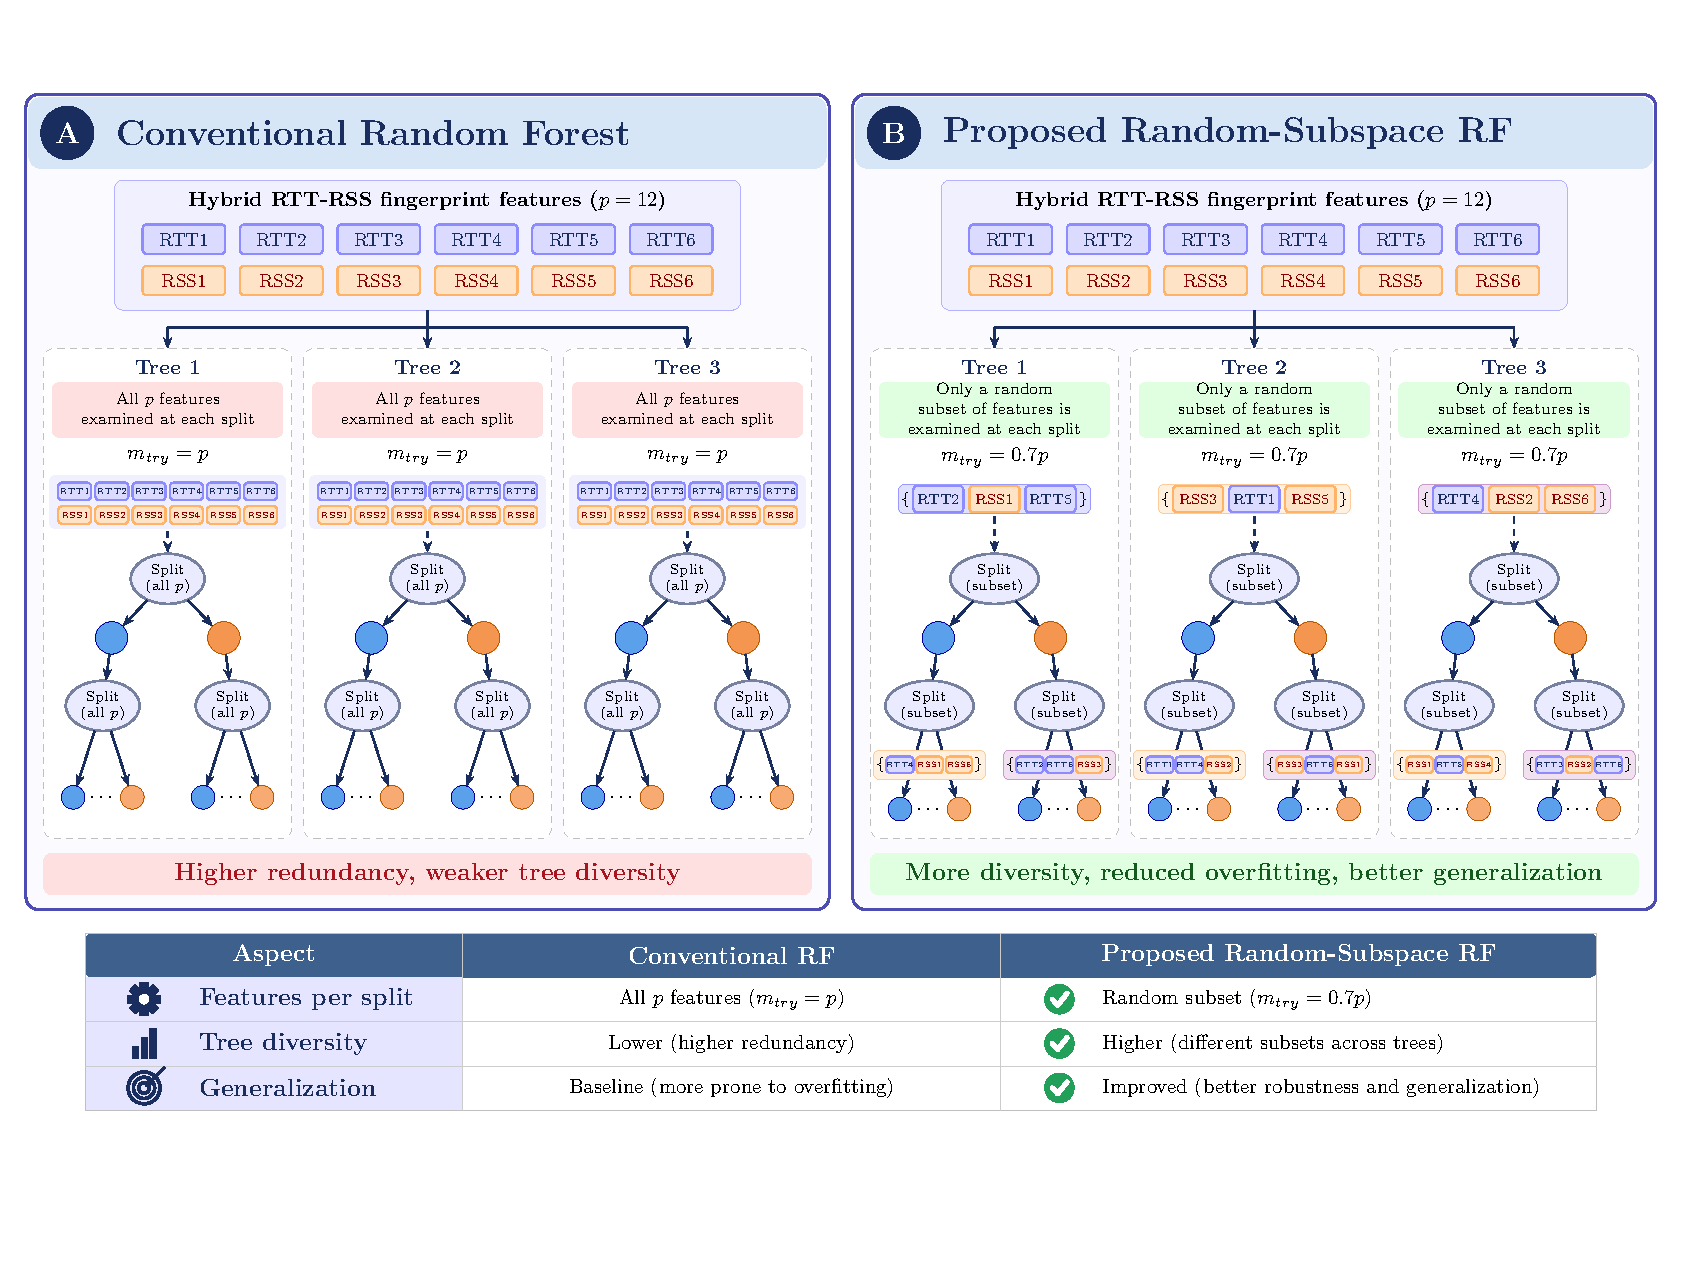
\includegraphics[width=\textwidth]{figures/methodology/fig03_rf_vs_subspace_rf.pdf}
	\caption{Conventional full-feature Random Forest and the proposed random-subspace Random Forest. In the conventional model, all $p$ hybrid RTT--RSS features are eligible at each split. The proposed model randomly exposes approximately $0.7p$ candidate features at each node, increasing ensemble diversity and reducing dependence on redundant or unstable measurements.}
	\label{fig:rf_subspace}
\end{figure*}

Per-split subsampling is a form of regularization whose optimal strength depends on the signal-to-noise ratio~\cite{mentch2020randomization}. Estimating positions between surveyed RPs is an interpolation problem that becomes noisier as the radio map becomes sparser. We therefore hypothesize that the optimal $\rho$ decreases with radio-map density; this is tested in Section~\ref{subsec:density_results}.

% ============================================================
\subsection{RP-Aware Validation}
\label{subsec:rp_grouping}

For grouped $K$-fold validation, the set of RP identifiers is partitioned into disjoint folds $\mathbb{G}^{(1)},\ldots,\mathbb{G}^{(K)}$; the model of fold $k$ is trained on all scans whose RP is not in $\mathbb{G}^{(k)}$ and predicts the scans of $\mathbb{G}^{(k)}$. Metrics are computed on the pooled out-of-fold predictions of all folds. Figure~\ref{fig:rp_validation} contrasts this protocol with sample-level splitting.

\begin{figure*}[!t]
	\centering
	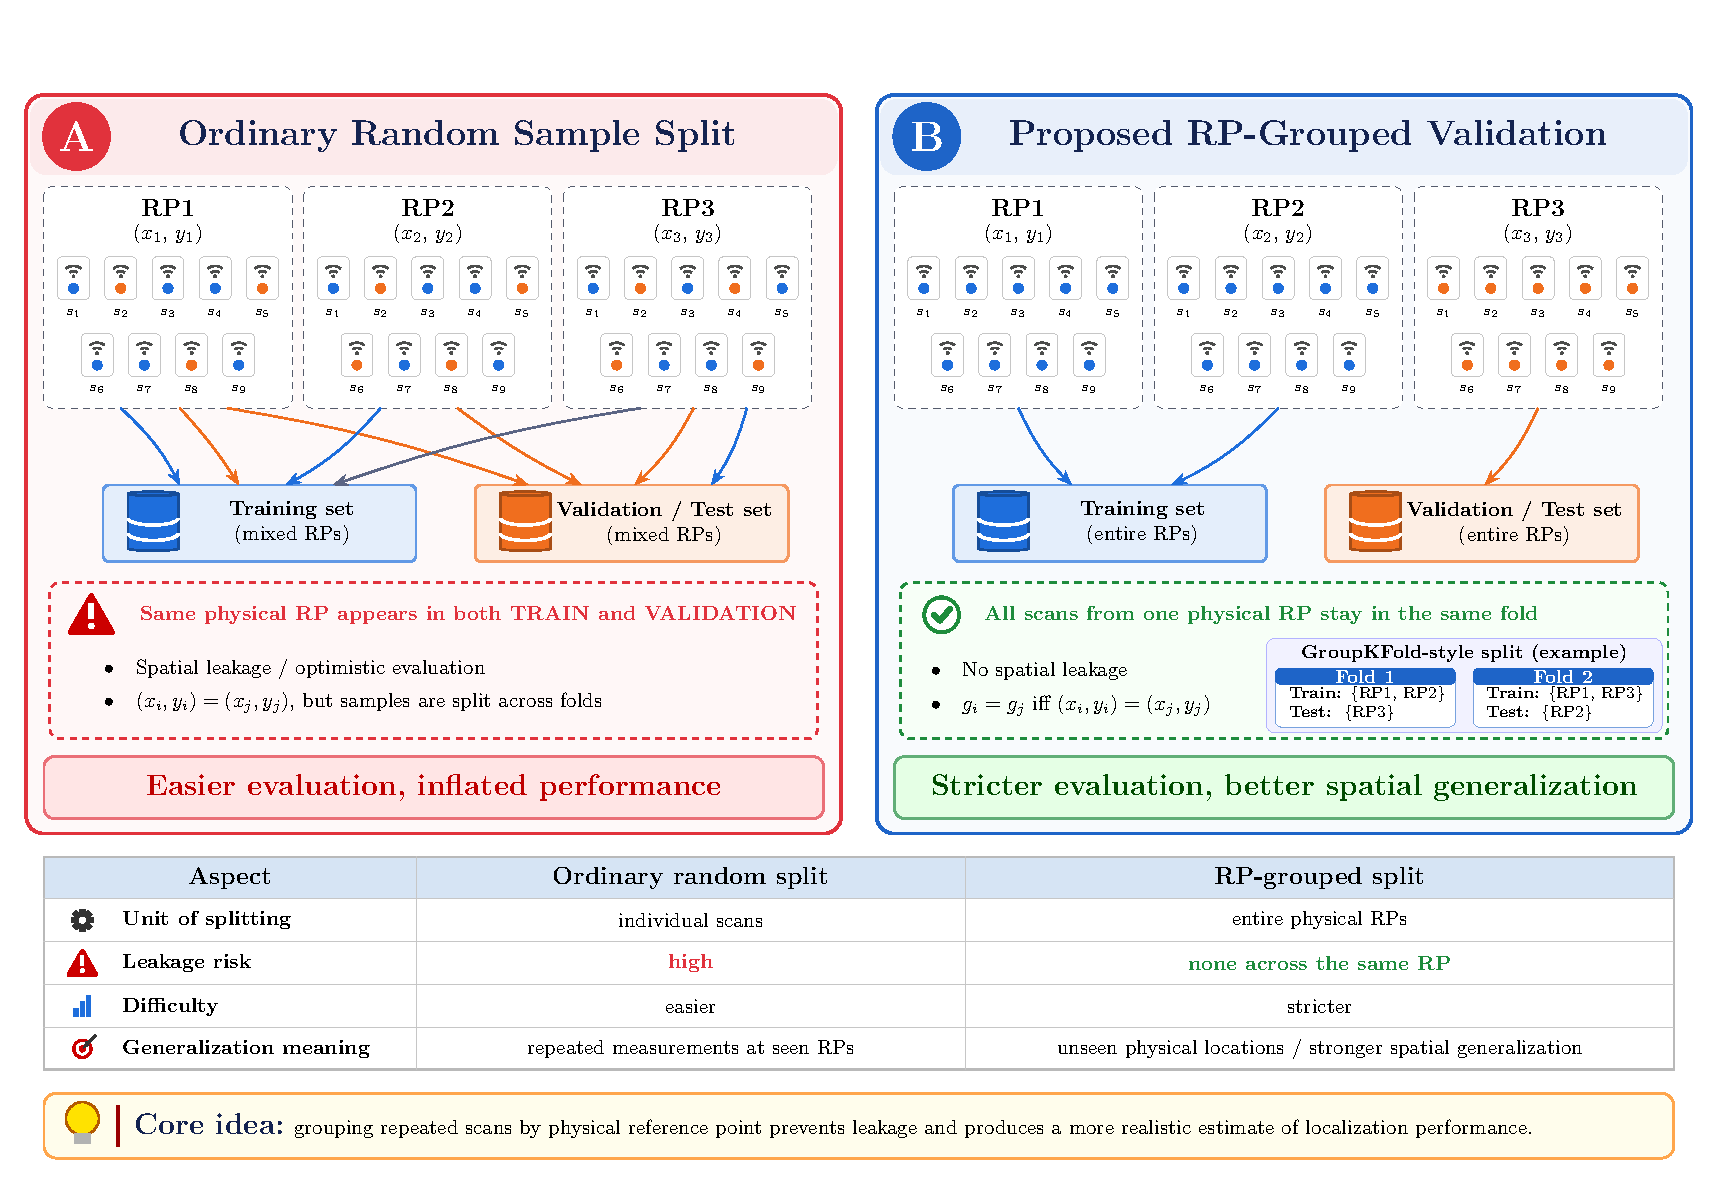
\includegraphics[width=\textwidth]{figures/methodology/fig04_rp_grouped_validation.pdf}
	\caption{Random sample-level splitting versus reference-point-aware validation. With row-level splitting, repeated scans collected at the same physical RP may appear in both training and validation subsets. RP-grouped validation keeps all measurements from one physical position in the same partition, enabling evaluation on physically unseen reference points.}
	\label{fig:rp_validation}
\end{figure*}

% ============================================================
\subsection{Choice of the Subspace Ratio}
\label{subsec:model_selection}

A natural way to select $\rho$ is to minimize a validation loss over a candidate set $\mathcal{R}$,
\begin{equation}
	\rho^{*}
	=
	\arg\min_{\rho\in\mathcal{R}}
	\mathcal{L}_{\mathrm{val}}(\rho),
	\label{eq:rho_selection}
\end{equation}
where $\mathcal{L}_{\mathrm{val}}$ is the out-of-bag (OOB) error of the forest, a sample-level $K$-fold cross-validation (CV) error, or an RP-grouped CV error. In fingerprinting, each estimator is biased in a specific way. OOB and sample-level CV evaluate each scan with trees trained on other scans of the same RP, so they measure fingerprint recognition and produce errors far below the test error. RP-grouped CV removes this leakage, but its fold models are trained on $(K-1)/K$ of the RPs, i.e., on a sparser radio map than the final model. If the optimal ratio depends on density, RP-grouped CV selects a ratio that is too small for the full-density model.

We therefore do not select $\rho$ by Eq.~\eqref{eq:rho_selection}. The proposed configuration uses the fixed default $\rho=0.7$, set during method development and frozen before external evaluation. Its quality is assessed afterwards by its regret on the official RP-disjoint test sets, with $\mathcal{L}_{\mathrm{test}}$ the paper-compatible error of Eq.~\eqref{eq:paper_metric},
\begin{equation}
	\mathrm{Regret}(\rho)
	=
	\frac{\mathcal{L}_{\mathrm{test}}(\rho)}{\min_{\rho'\in\mathcal{R}}\mathcal{L}_{\mathrm{test}}(\rho')}-1,
	\label{eq:regret}
\end{equation}
and compared with the regret of the data-driven rules above, of a leave-one-environment-out rule that picks the ratio minimizing the worst RP-grouped CV regret on the other environments, and of the defaults $\rho=1$ and $m_{\mathrm{try}}=\lfloor p/3\rfloor$~\cite{breiman2001random}. The test sets score these rules but never choose $\rho$.

After validation, the final model $f^{*}$ is trained on all available training RPs (Algorithm~\ref{alg:subspace_rf}), since every withheld RP makes the radio map sparser.

\begin{algorithm}[t]
	\caption{RP-Aware Random-Subspace RTT--RSS Localization}
	\label{alg:subspace_rf}
	\begin{algorithmic}[1]

		\Require
		Fingerprint dataset
		$\mathcal{D}=\{(\mathbf{z}_i,\mathbf{u}_i,g_i)\}_{i=1}^{N}$;
		number of trees $T$;
		fixed subspace ratio $\rho$ (default $0.7$);
		number of grouped folds $K$

		\Ensure
		Final positioning model $f^{*}$; RP-disjoint validation estimate

		\State $m_{\mathrm{try}} \leftarrow \max(1,\lfloor \rho p \rfloor)$

		\For{$k=1$ to $K$}
		\Comment{validation only}

		\State Construct RP-disjoint training and validation sets:
		$\mathcal{G}^{(k)}_{\mathrm{train}}\cap\mathcal{G}^{(k)}_{\mathrm{val}}=\varnothing$

		\State $f^{(k)} \leftarrow \mathrm{RF}\left(\mathcal{D}^{(-k)};\,T,\,m_{\mathrm{try}}\right)$

		\State $\hat{\mathbf{u}}_i^{\mathrm{OOF}} \leftarrow f^{(k)}(\mathbf{z}_i)$ for all $i$ with $g_i\in\mathcal{G}^{(k)}_{\mathrm{val}}$

		\EndFor

		\State Report metrics on the pooled out-of-fold predictions
		$\{\hat{\mathbf{u}}_i^{\mathrm{OOF}}\}_{i=1}^{N}$

		\State Train the final model on all available training RPs:
		\[
		f^{*}
		\leftarrow
		\mathrm{RF}
		\left(
		\mathcal{D};\,
		T,\,
		m_{\mathrm{try}}
		\right)
		\]

		\State \Return $f^{*}$

	\end{algorithmic}
\end{algorithm}


% ============================================================
\subsection{Grouped Out-of-Fold Residuals}
\label{subsec:oof_residual}

Uncertainty estimation requires residuals of predictions at locations the model has not seen. For each scan $i$, the RP-grouped out-of-fold prediction $\hat{\mathbf{u}}_{i}^{\mathrm{OOF}}$ is produced by the fold model that excluded the RP of $i$, and the residual is
\begin{equation}
	\boldsymbol{\epsilon}_{i}
	=
	\mathbf{u}_{i}-\hat{\mathbf{u}}_{i}^{\mathrm{OOF}}
	=
	\left[x_i-\hat{x}_i^{\mathrm{OOF}},\;y_i-\hat{y}_i^{\mathrm{OOF}}\right]^{T}.
	\label{eq:oof_residual}
\end{equation}

% ============================================================
\subsection{Circular and Covariance-Aware Elliptical Regions}
\label{subsec:circle_uncertainty}

The isotropic nonconformity score is $s_i^{\mathrm{circ}}=\|\boldsymbol{\epsilon}_{i}\|_{2}$, which yields the circular region
\begin{equation}
	\mathcal{C}_{\mathrm{circ}}
	=
	\left\{\mathbf{u}:\|\mathbf{u}-\hat{\mathbf{u}}^{*}\|_{2}\leq q_{\mathrm{circ}}\right\},
	\qquad
	A_{\mathrm{circ}}=\pi q_{\mathrm{circ}}^{2},
	\label{eq:circle_region}
\end{equation}
around a new prediction $\hat{\mathbf{u}}^{*}$, where $q_{\mathrm{circ}}$ is a calibrated quantile of the scores (Section~\ref{subsec:strict_conformal}).

Indoor errors are often anisotropic because of corridors, walls, and AP geometry. With the regularized residual covariance $\boldsymbol{\Sigma}=\mathrm{Cov}(\{\boldsymbol{\epsilon}_{i}\})+\lambda\mathbf{I}$, where $\lambda$ is a small ridge for numerical stability, the Mahalanobis score
\begin{equation}
	s_{i}^{\mathrm{ell}}
	=
	\sqrt{\boldsymbol{\epsilon}_{i}^{T}\boldsymbol{\Sigma}^{-1}\boldsymbol{\epsilon}_{i}}
	\label{eq:mahalanobis_score}
\end{equation}
yields the elliptical region (Fig.~\ref{fig:circle_ellipse})
\begin{align}
	\mathcal{C}_{\mathrm{ell}}
	&=
	\left\{\mathbf{u}:(\mathbf{u}-\hat{\mathbf{u}}^{*})^{T}\boldsymbol{\Sigma}^{-1}(\mathbf{u}-\hat{\mathbf{u}}^{*})\leq q_{\mathrm{ell}}^{2}\right\},
	\label{eq:ellipse_region}\\
	A_{\mathrm{ell}}
	&=
	\pi q_{\mathrm{ell}}^{2}\sqrt{\det\boldsymbol{\Sigma}}.
	\label{eq:ellipse_area}
\end{align}
A region is evaluated by its area together with its empirical coverage on the test set,
\begin{equation}
	\mathrm{Coverage}
	=
	\frac{1}{N_t}\sum_{i=1}^{N_t}\mathbb{I}\left[\mathbf{u}_{i}\in\mathcal{C}_{i}\right],
	\label{eq:coverage}
\end{equation}
and a smaller region is only better at equal coverage.

\begin{figure}[!t]
	\centering
	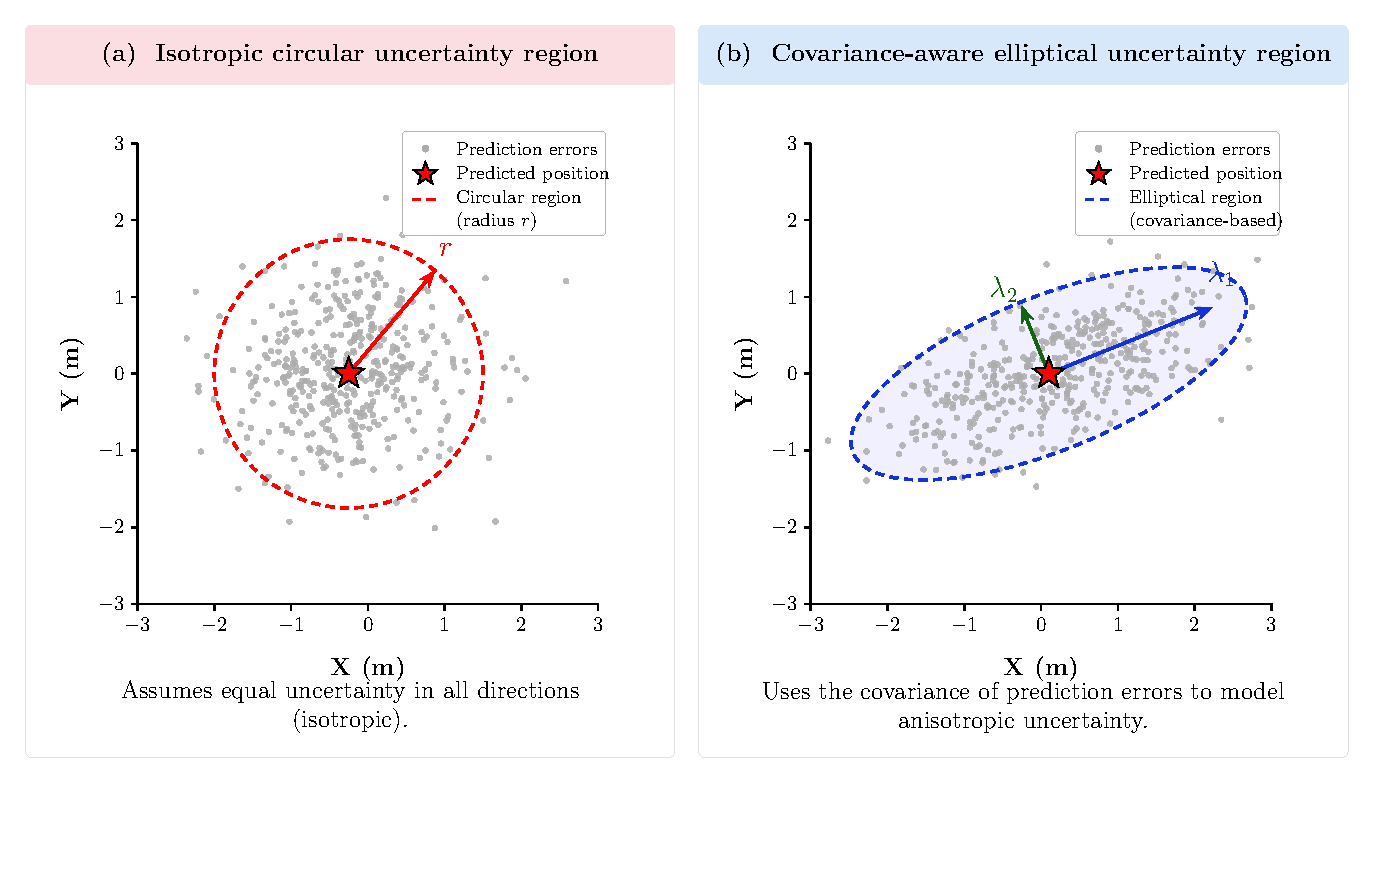
\includegraphics[width=\columnwidth]{figures/methodology/fig05_circle_vs_ellipse.pdf}
	\caption{Circular and covariance-aware elliptical uncertainty regions. The circular construction assigns the same uncertainty scale in every direction. The covariance-aware ellipse adapts its orientation and axis lengths according to the spatial covariance of localization residuals.}
	\label{fig:circle_ellipse}
\end{figure}

% ============================================================
\subsection{Calibration}
\label{subsec:strict_conformal}

\subsubsection{Scan-Level Split Conformal}
The training RPs are split into disjoint fitting and calibration sets, $\mathbb{G}_{\mathrm{fit}}\cap\mathbb{G}_{\mathrm{cal}}=\varnothing$. The point predictor is trained on $\mathcal{D}_{\mathrm{fit}}$, $\boldsymbol{\Sigma}$ is estimated from grouped OOF residuals inside $\mathcal{D}_{\mathrm{fit}}$, and the threshold, $q_{\mathrm{circ}}$ or $q_{\mathrm{ell}}$ depending on the score, is computed from the sorted scores $s_{(1)}\leq\cdots\leq s_{(n)}$ of the calibration scans,
\begin{equation}
	q_{\alpha}
	=
	s_{\left(\left\lceil(n+1)(1-\alpha)\right\rceil\right)},
	\label{eq:conformal_quantile}
\end{equation}
with $n=n_{\mathrm{cal}}$, the number of calibration scans. This is standard practice in conformal indoor positioning~\cite{feng2026robust}, and it gives the marginal coverage guarantee $P(\mathbf{u}\in\mathcal{C})\geq1-\alpha$ when calibration and test scans are exchangeable~\cite{lei2018distribution}.

\subsubsection{Group Split Conformal}
\label{subsubsec:group_conformal}
In fingerprinting, the calibration scans are not exchangeable with the test scans: they come from $G$ held-out RPs with $\sim$120 nearly identical scans each, whereas the test scans come from other RPs. The exchangeable units are the RPs, so the effective calibration sample size is $G$, not $n_{\mathrm{cal}}$. Following Dunn et al.~\cite{Dunn02102023}, we draw one scan at random from each calibration RP and apply Eq.~\eqref{eq:conformal_quantile} to these $G$ scores, i.e., with $n=G$. If the RPs are exchangeable, the score of one random scan of a new test RP is exchangeable with these $G$ scores, and the resulting region has the marginal coverage guarantee for a scan of a new RP. The guarantee holds on average over the calibration draw; individual calibration sets can cover more or less. The construction requires $\lceil(G+1)(1-\alpha)\rceil\leq G$, i.e., $G\geq1/\alpha-1$: at least 9 calibration RPs for $90\%$ and 19 for $95\%$. With fewer RPs, no finite distribution-free region exists.

\subsubsection{RP-Count Conservative Correction}
\label{subsubsec:rp_corrected}
As a simple alternative that uses all calibration scans, we also evaluate an RP-count-based correction that pools the scores but computes the finite-sample level from $G$:
\begin{align}
	q_{\alpha}^{\mathrm{RP}}
	&=
	Q_{\ell_G}\!\left(\{s_1,\ldots,s_{n_{\mathrm{cal}}}\}\right),
	\label{eq:rp_corrected_quantile}\\
	\ell_G
	&=
	\min\!\left(1,\frac{\lceil (G+1)(1-\alpha)\rceil}{G}\right),
	\label{eq:rp_level}
\end{align}
where $Q_{\ell}$ is the empirical $\ell$-quantile (``higher'' interpolation). Because $\ell_G$ is never smaller than the scan-level level, $q_{\alpha}^{\mathrm{RP}}\geq q_{\alpha}$. This correction is a conservative heuristic without a finite-sample guarantee, and it is evaluated empirically. When $G<2/\alpha-1$ (fewer than 19 calibration RPs at $90\%$ or 39 at $95\%$), $\ell_G=1$ and the threshold becomes the largest calibration score.

\subsubsection{Full-Training Grouped-OOF Variant}
\label{subsec:empirical_oof}
Reserving calibration RPs costs point accuracy. In this variant, the final predictor is trained on all training RPs, and $\boldsymbol{\Sigma}$ and the thresholds are computed from the grouped OOF residuals of Section~\ref{subsec:oof_residual}. Because these residuals come from several fold models rather than from one predictor and an independent calibration set, the variant is an empirical estimator without the split-conformal guarantee; cross-fitted constructions such as CV+ would be required for one~\cite{barber2021jackknife}. The procedure is summarized in Algorithm~\ref{alg:uncertainty}.

\begin{algorithm}[t]
	\caption{RP-Grouped Covariance-Aware Uncertainty Estimation}
	\label{alg:uncertainty}
	\begin{algorithmic}[1]
		
		\Require
		Training dataset
		$\mathcal{D}=\{(\mathbf{z}_i,\mathbf{u}_i,g_i)\}_{i=1}^{N}$;
		number of folds $K$;
		confidence level $1-\alpha$;
		fixed RF parameters $T=300$ and $\rho=0.7$
		
		\Ensure
		Residual covariance $\boldsymbol{\Sigma}$;
		circular threshold $q_{\mathrm{circ}}$;
		elliptical threshold $q_{\mathrm{ell}}$
		
		\State Partition physical RPs into $K$ disjoint groups
		
		\For{$k=1$ to $K$}
		
		\State Train the fold model without RP group $k$:
		\[
		f^{(-k)}
		\leftarrow
		\mathrm{RF}
		\left(
		\mathcal{D}^{(-k)};
		300,
		0.7
		\right)
		\]
		
		\For{each sample $i$ in held-out RP fold $k$}
		
		\State Compute out-of-fold prediction:
		\[
		\hat{\mathbf{u}}_i^{\mathrm{OOF}}
		=
		f^{(-k)}(\mathbf{z}_i)
		\]
		
		\State Compute residual:
		\[
		\boldsymbol{\epsilon}_i
		=
		\mathbf{u}_i
		-
		\hat{\mathbf{u}}_i^{\mathrm{OOF}}
		\]
		
		\EndFor
		
		\EndFor
		
		\State Estimate residual covariance:
		\[
		\boldsymbol{\Sigma}
		=
		\mathrm{Cov}
		\left(
		\{\boldsymbol{\epsilon}_i\}
		\right)
		+
		\lambda\mathbf{I}
		\]
		
		\For{each residual $\boldsymbol{\epsilon}_i$}
		
		\State Circular score:
		\[
		s_i^{\mathrm{circ}}
		=
		\|\boldsymbol{\epsilon}_i\|_2
		\]
		
		\State Elliptical score:
		\[
		s_i^{\mathrm{ell}}
		=
		\sqrt{
			\boldsymbol{\epsilon}_i^{T}
			\boldsymbol{\Sigma}^{-1}
			\boldsymbol{\epsilon}_i
		}
		\]
		
		\EndFor
		
		\State Compute uncertainty thresholds with the finite-sample level of Eq.~\eqref{eq:conformal_quantile}, $n=N$:
		\[
		q_{\mathrm{circ}}
		=
		s^{\mathrm{circ}}_{\left(\lceil (N+1)(1-\alpha)\rceil\right)},
		\qquad
		q_{\mathrm{ell}}
		=
		s^{\mathrm{ell}}_{\left(\lceil (N+1)(1-\alpha)\rceil\right)}
		\]
		
		\State \Return
		$\boldsymbol{\Sigma}$,
		$q_{\mathrm{circ}}$,
		$q_{\mathrm{ell}}$
		
	\end{algorithmic}
\end{algorithm}

% ============================================================
\subsection{Computational Complexity}
\label{subsec:complexity}

Training an RF costs approximately $\mathcal{O}(T N m_{\mathrm{try}}\log N)$ for $N$ training scans, so $\rho=0.7$ reduces the number of candidate-feature evaluations per split by $30\%$; measured wall-clock times also depend on tree depth, parallelization, and implementation and are therefore reported explicitly. Inference traverses one root-to-leaf path per tree, $\mathcal{O}(T D_t)$ for average depth $D_t$, so model size and latency are controlled mainly by $T$ and the leaf size. Grouped fold models are needed only offline. Online, the system evaluates $f^{*}$ and, if requested, returns $\mathcal{C}_{1-\alpha}$, which adds only a two-dimensional quadratic form.
